\documentclass[11pt]{article}
\usepackage[
top    = 2.50cm,% presumably you don't want it to be 0pt as well?
bottom = 2.50cm,
left   = 2cm,
right  = 2cm,
marginparsep = 0pt,
marginparwidth=0pt,
]{geometry}

\usepackage{amssymb}
\usepackage{fancyhdr}
\usepackage[most]{tcolorbox}
\usetikzlibrary{calc}
\usepackage{siunitx}
\usepackage{amsmath}
\usepackage{tikz}
\usepackage{caption}
\usepackage{pgfplots}
\usepackage{multicol}
\pagestyle{fancy}
\fancyhead[l]{Mechanics: Dynamics - Abridged edition}
\fancyhead[r]{Giorgio G.}
\newcommand\findtan[2][3]{
	\pgfmathtruncatemacro\glen{#1/3*2}
	\node[coordinate, label={#2:$A$}] (p) at (#2:#1 cm) {};
	\draw[ultra thick, blue, <-] (c) -- (p);
	\path ($(c)!.5!(p)$) --++ (-90+#2:3mm) node[at end] {$F_c$};
	\draw[ultra thick, green, ->] (p) -- ++(90+#2:\glen cm) coordinate (e); 
	\path (e) --++ (0+#2:4mm) node[at end] {$v$};
}
\begin{document}
	
	\section{The Laws of Motion: }
	
	
	
	\subsection{Newton's 1\textsuperscript{st} Law}
	\begin{center}
		A body is either at rest, or moving with constant speed in a straight line, if no resultant force acts on it.
	\end{center}
	
	\begin{equation}
		p=mv\tag{\si{\kilogram\meter\per\second}}	
	\end{equation}	
	
	\begin{center}
		Where $p$ is an object's \textbf{momentum} (\si{\kilogram\meter\per\second}), $m$ its \textbf{mass} (\si{\kilogram}) and $v$ its \textbf{velocity} (\si{\meter\per\second}).
	\end{center}
	
	\subsection{Newton's 2\textsuperscript{nd} Law}
	\begin{center}
		The acceleration of a body is directly proportional to the resultant force applied to it  and acts in the same direction.
	\end{center}
	
	\begin{equation}
		F=ma \tag{\si{\newton}}	
	\end{equation}	
	
	\begin{center}
		Where $p$ is an object's \textbf{momentum} (\si{\kilogram\meter\per\second}), $m$ its \textbf{mass} (\si{\kilogram}) and $v$ (\si{\meter\per\second}) its \textbf{velocity}.
	\end{center}
	
	
	\subsection{Newton's 3\textsuperscript{rd} Law}
	\begin{center}
		To every action there is an equal and opposite reaction.
	\end{center}
	\begin{center}
		Consider object $A$ and object $B$:
	\end{center}
	
	\begin{equation}
		_AF_B =\\  _BF_A\tag{\si{\newton}}
	\end{equation}
	
	
	\section{Force of impact: }
	\begin{equation}
		F_i =\frac{mv-mu}{t}\tag{\si{\newton}}
	\end{equation}
	
	\section{Inclined plane: }
	
	\begin{multicols}{2}
		\begin{center}
			\underline{\textbf{Parallel}}
		\end{center}
		\begin{equation}
			mg\sin\theta\tag{\si{\newton}}
		\end{equation}
		\begin{center}
			\underline{\textbf{Perpendicular}}
		\end{center}
		\begin{equation}
			mg\cos\theta\tag{\si{\newton}}
		\end{equation}
		
	\end{multicols}
	
	\section{Conservation of momentum: }
	
	\begin{equation}
		Mu_1 + mu_2 = Mv_1 + mv_2\notag
	\end{equation}
	\begin{center}
		Where $M$ and $m$ are object 1 and 2's \textbf{masses} (\si\kilogram) respectively whilst $u$ and $v$ the initial and final \textbf{velocities} (\si{\meter\per\second}) of a given object respectively. 
	\end{center} 
	\newpage
	\section{Centripetal force: }
	\begin{center}
		
		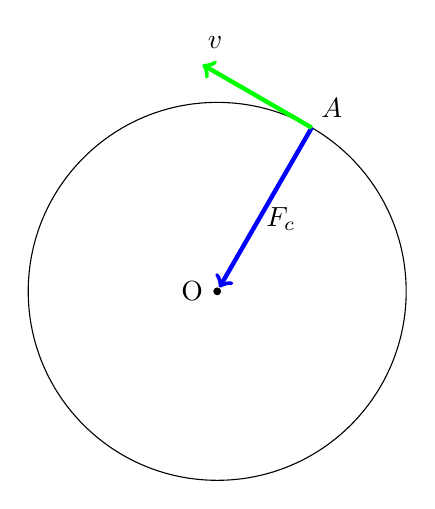
\begin{tikzpicture}[scale=0.8]
			\draw (0,0) circle (3cm);
			\node[circle,fill, inner sep=1pt, label={left:O}] (c) at (0,0) {};
			\findtan{60}
		\end{tikzpicture}
	\end{center}
	
	\begin{equation}
		F_c = \frac{mv^2}{r}\tag{\si{\newton}}
	\end{equation}
	\begin{center}
		Where $m$ is the given object's \textbf{mass} (\si{\kilogram}), $v$ its \textbf{tangential velocity}\footnote{The velocity perpendicular to the cirular path's radius.} (\si{\meter\per\second}) and $r$ the \textbf{radius} (\si{\meter}) of the cirular path.
	\end{center}
\subsection{Specific cases: }

	
		\begin{multicols}{2}
	\begin{center}
			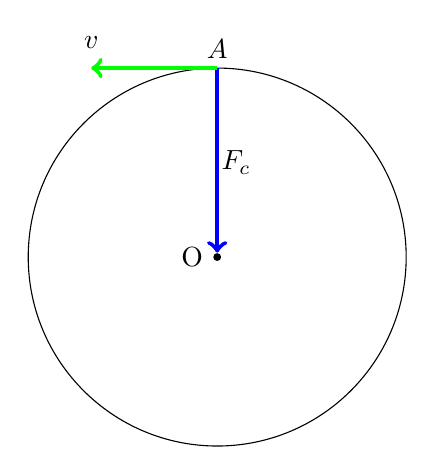
\begin{tikzpicture}[scale=0.8]
		\draw (0,0) circle (3cm);
		\node[circle,fill, inner sep=1pt, label={left:O}] (c) at (0,0) {};
		\findtan{90}
	\end{tikzpicture}
\begin{equation}
	F_c = \frac{mv^2}{r} =mg+R\notag
\end{equation}
	\end{center}
\begin{center}
		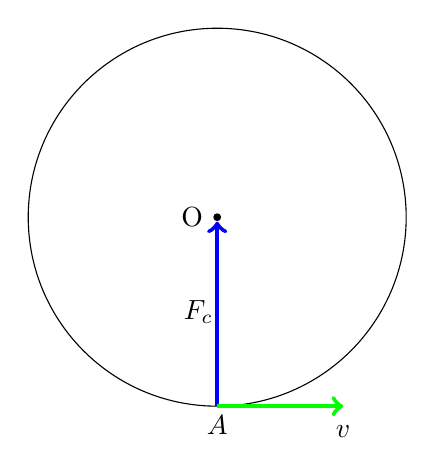
\begin{tikzpicture}[scale=0.8]
		\draw (0,0) circle (3cm);
		\node[circle,fill, inner sep=1pt, label={left:O}] (c) at (0,0) {};
		\findtan{270}
	\end{tikzpicture}\\
\begin{equation}
	F_c = \frac{mv^2}{r} =mg-R\notag
\end{equation}
\end{center}
\end{multicols}

	
	
\end{document}